
%%%%%%%%%%%%%%%%%%%%%%%%%%%%%%%%%%%%%%%%%%%%%%%%%%%%%%%%%%%%%%%%%%%%%%%%%%%%%%%%%%%%%%%
%%%%%%%%%%%%%%%%%%%%%%%%%%%%%%%%%%%%%%%%%%%%%%%%%%%%%%%%%%%%%%%%%%%%%%%%%%%%%%%%%%%%%%%
% 
% This top part of the document is called the 'preamble'.  Modify it with caution!
%
% The real document starts below where it says 'The main document starts here'.

\documentclass[12pt]{article}

\usepackage{amssymb,amsmath,amsthm}
\usepackage[top=1in, bottom=1in, left=1.25in, right=1.25in]{geometry}
\usepackage{fancyhdr}
\usepackage{enumerate}
\usepackage{listings}
\usepackage{graphicx}
\usepackage{float}

\usepackage{mwe}
\usepackage{caption}
\usepackage{subcaption}
% Comment the following line to use TeX's default font of Computer Modern.
\usepackage{times,txfonts}



\makeatletter
\renewcommand*\env@matrix[1][*\c@MaxMatrixCols c]{%
  \hskip -\arraycolsep
  \let\@ifnextchar\new@ifnextchar
  \array{#1}}
\makeatother

\newtheoremstyle{homework}% name of the style to be used
  {18pt}% measure of space to leave above the theorem. E.g.: 3pt
  {12pt}% measure of space to leave below the theorem. E.g.: 3pt
  {}% name of font to use in the body of the theorem
  {}% measure of space to indent
  {\bfseries}% name of head font
  {:}% punctuation between head and body
  {2ex}% space after theorem head; " " = normal interword space
  {}% Manually specify head
\theoremstyle{homework} 

% Set up an Exercise environment and a Solution label.
\newtheorem*{exercisecore}{Exercise \@currentlabel}
\newenvironment{exercise}[1]
{\def\@currentlabel{#1}\exercisecore}
{\endexercisecore}

\newcommand{\localhead}[1]{\par\smallskip\noindent\textbf{#1}\nobreak\\}%
\newcommand\solution{\localhead{Solution:}}

%%%%%%%%%%%%%%%%%%%%%%%%%%%%%%%%%%%%%%%%%%%%%%%%%%%%%%%%%%%%%%%%%%%%%%%%
%
% Stuff for getting the name/document date/title across the header
\makeatletter
\RequirePackage{fancyhdr}
\pagestyle{fancy}
\fancyfoot[C]{\ifnum \value{page} > 1\relax\thepage\fi}
\fancyhead[L]{\ifx\@doclabel\@empty\else\@doclabel\fi}
\fancyhead[C]{\ifx\@docdate\@empty\else\@docdate\fi}
\fancyhead[R]{\ifx\@docauthor\@empty\else\@docauthor\fi}
\headheight 15pt

\def\doclabel#1{\gdef\@doclabel{#1}}
\doclabel{Use {\tt\textbackslash doclabel\{MY LABEL\}}.}
\def\docdate#1{\gdef\@docdate{#1}}
\docdate{Use {\tt\textbackslash docdate\{MY DATE\}}.}
\def\docauthor#1{\gdef\@docauthor{#1}}
\docauthor{Use {\tt\textbackslash docauthor\{MY NAME\}}.}
\makeatother

% Shortcuts for blackboard bold number sets (reals, integers, etc.)
\newcommand{\Reals}{\ensuremath{\mathbb R}}
\newcommand{\Nats}{\ensuremath{\mathbb N}}
\newcommand{\Ints}{\ensuremath{\mathbb Z}}
\newcommand{\Rats}{\ensuremath{\mathbb Q}}
\newcommand{\Cplx}{\ensuremath{\mathbb C}}
%% Some equivalents that some people may prefer.
\let\RR\Reals
\let\NN\Nats
\let\II\Ints
\let\CC\Cplx
%%%%%%%%%%%%%%%%%%%%%%%%%%%%%%%%%%%%%%%%%%%%%%%%%%%%%%%%%%%%%%%%%%%%%%%%%%%%%%%%%%%%%%%
%%%%%%%%%%%%%%%%%%%%%%%%%%%%%%%%%%%%%%%%%%%%%%%%%%%%%%%%%%%%%%%%%%%%%%%%%%%%%%%%%%%%%%%
% 
% The main document start here.

% The following commands set up the material that appears in the header.




%  \textbf{Code:}
%  \begin{center}
%  \lstinputlisting[basicstyle = \footnotesize]{}
%  \end{center}
%  
%  \begin{footnotesize}
%  \begin{verbatim}
%    
%  \end{verbatim}
%  \end{footnotesize}
%  
%  
%  \begin{figure}[H]
%    \begin{center}
%      \caption{}
%    \includegraphics[width = \textwidth]{}
%    \end{center}
%  \end{figure}




\doclabel{Stat 461: Homework 6}
\docauthor{Stefano Fochesatto}
\docdate{March 6, 2022}

\begin{document}
\begin{exercise}{1} Use the following code to read in the Harvard Forest Dataset HF143 Data. It is in the file 
  datasoil.txt. It consists of soil properties along three transects in Harvard Forest, collected by Richard Bowden, 
  Charles McClaugherty and, Timothy Sipe. \\
  \begin{enumerate}
    \item[a.] Look at the output. Is a decent amont of the variability explained by the first 4 factors? Use the test of hypothesis of 
    sufficient numbers of factors to find a suitable number of factors to use. What proportion of the variability in the data is explained by the 
    factor analysis?\\
    \solution Cleaning the data, we exclude the first four columns since they are not numerical. The first column of data ff.thickness seems to have a lot of missing values.
    Experimenting with how we can clean up the data, I found that trying to impute the missing values ff.thickness with the mean, MLR estimation or even just removing the whole column we were able to retain a lot of 
    the observations. Unfortunately It seems as though with 300 plus observations the factor analysis algorithm becomes unstable (I'd imagine it is problematic for the cholesky-esque factorization that is needed to compute the loadings).
    So I ended up just removing the first four columns and removing any observations with NAs, reducing the number of observations to 155. 
    
    Running the factor analysis with for 4 factors, with varimax rotation, we find that the data is highly variable (at least when we consider only orthogonal rotations)
    since the first and largest factor only explains 16.4\% of the variance, with only about 44\% of the variance being explained by the first four factors. The factor analysis with only 4 factors rejects the 
    hypothesis that 4 factors are sufficient with a p-value of 4.43e-12. Interestingly a minimum of 8 factors were necessary in order to accept the null hypothesis at an $\alpha = .05$, In that case it's clear that adding more factors 
    is explaining the variance little by little, until we've explained a majority of the variance.\\
      \textbf{Code:}
      \begin{center}
      \lstinputlisting[basicstyle = \footnotesize]{r1.txt}
      \end{center}

    \vspace{.15in}



    \item[b.] Look at the factor loading. Can you roughly interpret the loadings on the first factor? Is it always possible to do so? Why or why not?\\
    \solution Looking at the magnitudes of the loadings we find that the first factor seems to heavily emphasize the c,n, and om variables. Looking at the documentation provided by the 
    data we can see that theses variables correspond to percent carbon, percent nitrogen, and percent organic matter. Given that these are primary factors in evaluating soil health/fertility, it seems like 
    this first factor maybe telling us this about our data. It is not always possible to interpret the loadings on any of the factors, most of the time the first factor will be the easiest to interpret, as it 
    captures the most variance (is able to most of the signal in the data). It really depends on the signal to noise ratio that is found in the data. Data that are entirely noise will result in practically useless, uninterpretable loadings
    \vspace{.15in}  

    \item[c.] Try a promax rotation, What is this and how does it differ from varimax rotation? Did the proportion of variation explained or the hypothesis test 
    change by much? Why is this result reasonable? Why did it show factor correlations for promax and not for varimax?. \\
    \solution Using the promax parameter allows for non-orthogonal factors. Generally when we do factor analysis, we want to generate the following factorization for our data $X$, 
    \begin{equation*}
      X = L'F+E
    \end{equation*}
    With varimax the columns of $F$ are orthogonal, with promax the columns of $F$ are allowed to be non-orthogonal. Performing the factor analysis with promax rotation we find that, allowing for non-orthogonal factors does not significantly effect 
    the analysis with respect to the amount of variance explained, and similarly we need 8 factors in order to accept the null hypothesis at an $\alpha = .05$. Factor correlations are displayed by promax because, in this case the factors are allowed to be correlated because 
    of the non-orthogonality.\\
    \textbf{Code:}
    \begin{center}
    \lstinputlisting[basicstyle = \footnotesize]{r2.txt}
    \end{center}
    \vspace{.15in}


    \item[d.] What does the plot of scores tell you? What are scores?\\
    \solution Scores of an observations we can see how much of each factor influences it. Considering the score plots, we can see any trends among the factors as well as to see if any outliers 
    have affected our factor analysis. With both factor analysis' there do not appear to be extreme outliers which define each factor. There seems to be a grouping of observations with high 1 factor scores, however the 
    factor does not seem to be defined by outliers, there is a good spread of observations across both factors. 
      \begin{figure}[H]
        \begin{center}
          \caption{Varimax Score Plot}
        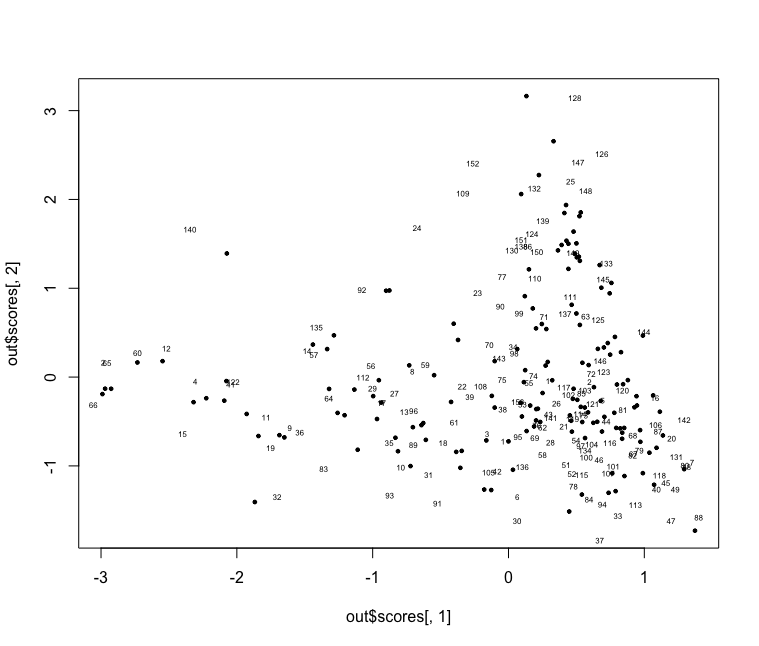
\includegraphics[width = .75\textwidth]{Rplot.png}
        \end{center}
      \end{figure}

      \begin{figure}[H]
        \begin{center}
          \caption{Promax Score Plot}
        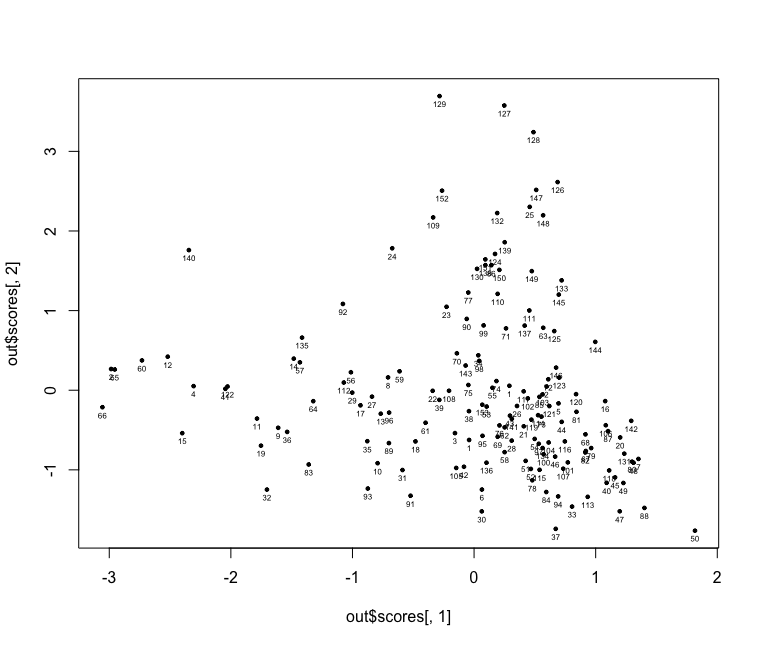
\includegraphics[width = .75\textwidth]{Rplot01.png}
        \end{center}
      \end{figure}
    \end{enumerate}
\end{exercise}
\vspace{1in} 



\begin{exercise}{2} Using the same dataset as in problem one, run a principal components analysis. Use a screeplot to select the number of important PCs. 
  Do the number of PCs seem to match what you got with the factor analysis. Do the loadings look similar ot those from the factors you calculated in b and c?
  Why do you think this happened?\\
  \solution Performing the principal component analysis we get the following screeplot. Considering the 'keep PCs' which contribute to 10 percent or more of the variance explained we 
  see that PCA gives us around 8 or 9 components. This agrees with our factor analysis. Considering the loadings, from the PCA we do see some similarity among the first factor, with respect to the 
  loadings from the factor analysis.
  \begin{figure}[H]
    \begin{center}
      \caption{PCA Scree Plot}
    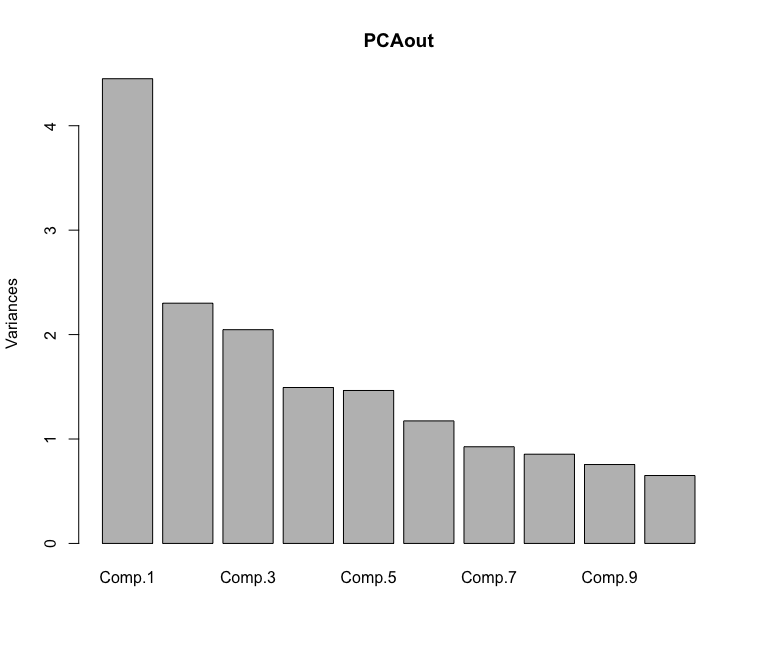
\includegraphics[width = .75\textwidth]{Rplot02.png}
    \end{center}
  \end{figure}
  \textbf{Code:}
  \begin{center}
  \lstinputlisting[basicstyle = \footnotesize]{r3.txt}
  \end{center}
  \vspace{.15in}

  
  
  
  We see that the first component of the PCA again favors variables c, n, and om similarly to the factor analysis loadings. The rest of the loadings do not look particularly
  similar. This makes sense that they are not exactly the same. PCA generates loadings by solving the eigenvalue eigenvector problem on the correlation matrix, factor analysis generates loadings via an 
  algorithm which minimizes the error in the following factorization, 
  \begin{equation*}
    \Sigma_x = LL' + D. 
  \end{equation*}
  
\end{exercise}
\vspace{1in} 





\begin{exercise}{3} Below is the covariance matrix based on $N = 150$ first year college students.  

  \begin{footnotesize}
  \begin{verbatim}
    M <-
    structure(c(0.594, 0.483, 3.993, 0.426, 0.5, 0.483, 0.754, 3.626,
    1.757, 0.722, 3.993, 3.626, 47.457, 4.1, 6.394, 0.426, 1.757,
    4.1, 10.267, 0.525, 0.5, 0.722, 6.394, 0.525, 2.675), .Dim = c(5L,
    5L), .Dimnames = list(c("GPAreq", "GPAelec", "SAT", "IQ", "EdMot"
    ), c("GPAreq", "GPAelec", "SAT", "IQ", "EdMot")))
  \end{verbatim}
  \end{footnotesize}
  \begin{enumerate}
    \item[a.] Try to make up two or three reasonable path analysis models for this data. Draw a structural diagram for each. Also, list 
    all of the parameters of each model.\\
    \solution Here is my first attempt at a structural diagram. It seems as though IQ and EdMot are exogenous variables, they seem to be outside variables 
    used for predicting student success in metrics like GPA, and SAT scores. In this case we have six regression parameters, three error variances, and three covariances. This is 
    the following structural diagram, 
    \begin{figure}[H]
      \begin{center}
        \caption{First Structural Diagram}
      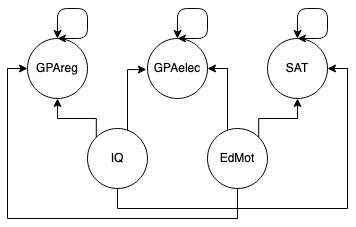
\includegraphics[width = .65\textwidth]{FirstDiagram.png}
      \end{center}
    \end{figure}
    My second structural diagram uses school performance metrics like GPA and SAT scores to predict IQ and EdMot, sort of the inverse of the previous diagram. Here we assume that 
    GPA, and SAT Scores are exogenous and IQ and EdMot are endogenous(seems unlikely but we'll test it anyway). This structural diagram has six regression parameters, two error variances, and one covariance. 
    \begin{figure}[H]
      \begin{center}
        \caption{Second Structural Diagram}
      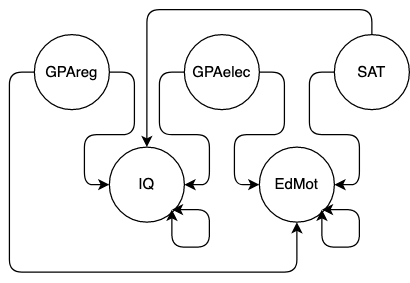
\includegraphics[width =  .65\textwidth]{SecondDiagram.png}
      \end{center}
    \end{figure}
    My third structural diagram uses GPA to predict IQ, EdMot, and SAT Scores. In this model we are treating GPA as an exogenous variable and the rest as endogenous. This model continues 
    six regression parameters and three error variances, and three covariances.
    \begin{figure}[H]
      \begin{center}
        \caption{Third Structural Diagram}
      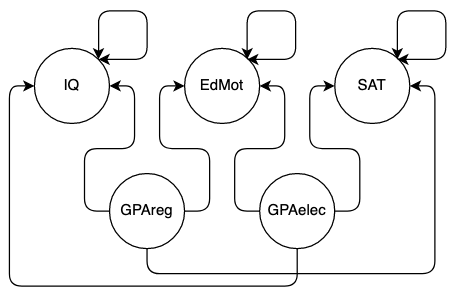
\includegraphics[width =  .65\textwidth]{ThirdDiagram.png}
      \end{center}
    \end{figure}



    \vspace{,15in}
    
    
    \item[b,] Using lavaan, run each model. Which model seems to fit the data best? how good is the fit of the model?\\
    \solution Calling AIC on the fitted models we find that the second structure diagram has the best fit. Interestingly this 
    is the model with the least degrees of freedom/parameters. All models had Standardized Root Mean Square Residual of 0 and CFI and TLI goodness 
    of fit values of 1.\\
    \textbf{Code:}
    \begin{center}
    \lstinputlisting[basicstyle = \footnotesize]{r4.txt}
    \end{center}
    \vspace{.15in}


    \item[c.] In your best fitting model, are any of the links candidates for removal? How could you determine this?\\
    \solution From the summary report we can see that the link between SAT and IQ can likely be a candidate for removal. The MLR which produces 
    IQ finds that the SAT variable has a p-value of 0.753, considerably higher than the rest and insignificant at the $\alpha = .05$ level. 
    \vspace{.15in}


    \item[d.] Why can't we use bootsrapping to get standard errors in this situation?\\
    \solution In this situation we don't have the data, only the covariance/correlation matrix.
    \vspace{.15in}


    \item[e.] Is the model you selected at best recursive, or non-recursive? How can you tell?\\
    \solution All of the models I selected are non-recursive. We setup up multiple regressions, and none of the results of those regressions feed into other regressions causing a loop or indirect effects. 
    \vspace{.15in}
    
    
    \item[f.] Are there any indirect effects in your best model? What are they?\\
    \solution My model has no indirect effects, IQ is directly modeled with GPA, and SAT and similarly with EdMot. 
    \vspace{.15in}
    
    \item[g,] What variables in your best model are exogenous, and which are endogenous?\\
    \solution Like previously stated the second model has GPA and SAT scores as exogenous variables and IQ and EdMot are endogenous.
    \vspace{.15in} 
  \end{enumerate}










\end{exercise}




\end{document}


















